\section{0{\nbb} decay vs $^{10}$C background}

Other common backgrounds to 0{\nbb} decay search include radioactive
decays of nuclei that are excited by cosmic muons and produced through the decays of Th and U
naturally present in the materials. In liquid scintillator detectors,
most of events from Th and U decays occur in the materials of
the scintillator enclosure. Typically, they enter the fiducial volume
as 2.6~MeV gammas. These gammas pass into the fiducial volume either because they showered too late or have
mis-reconstructed vertex. Both effects depend on details of a
particular experiment and in this paper we make no attempt
to introduce a topology reconstruction for the backgrounds coming from
Th and U lines. Cosmic induced backgrounds, to the contrary, are more
generic and originate inside the fiducial volume. In this section we
discuss event topology of $^{10}$C events that are most relevant in the
energy of 2-3~MeV.

Typical energy deposition by $^{10}$C events is shown in
Fig.~\ref{fig:Edep_C10}. We propose to use spherical harmonics
analysis to separate 0{\nbb} decay events from $^{10}$C events that
within energy resolution overlap with the 0{\nbb} decay Q-value.

\begin{figure}[h]
  \centering
  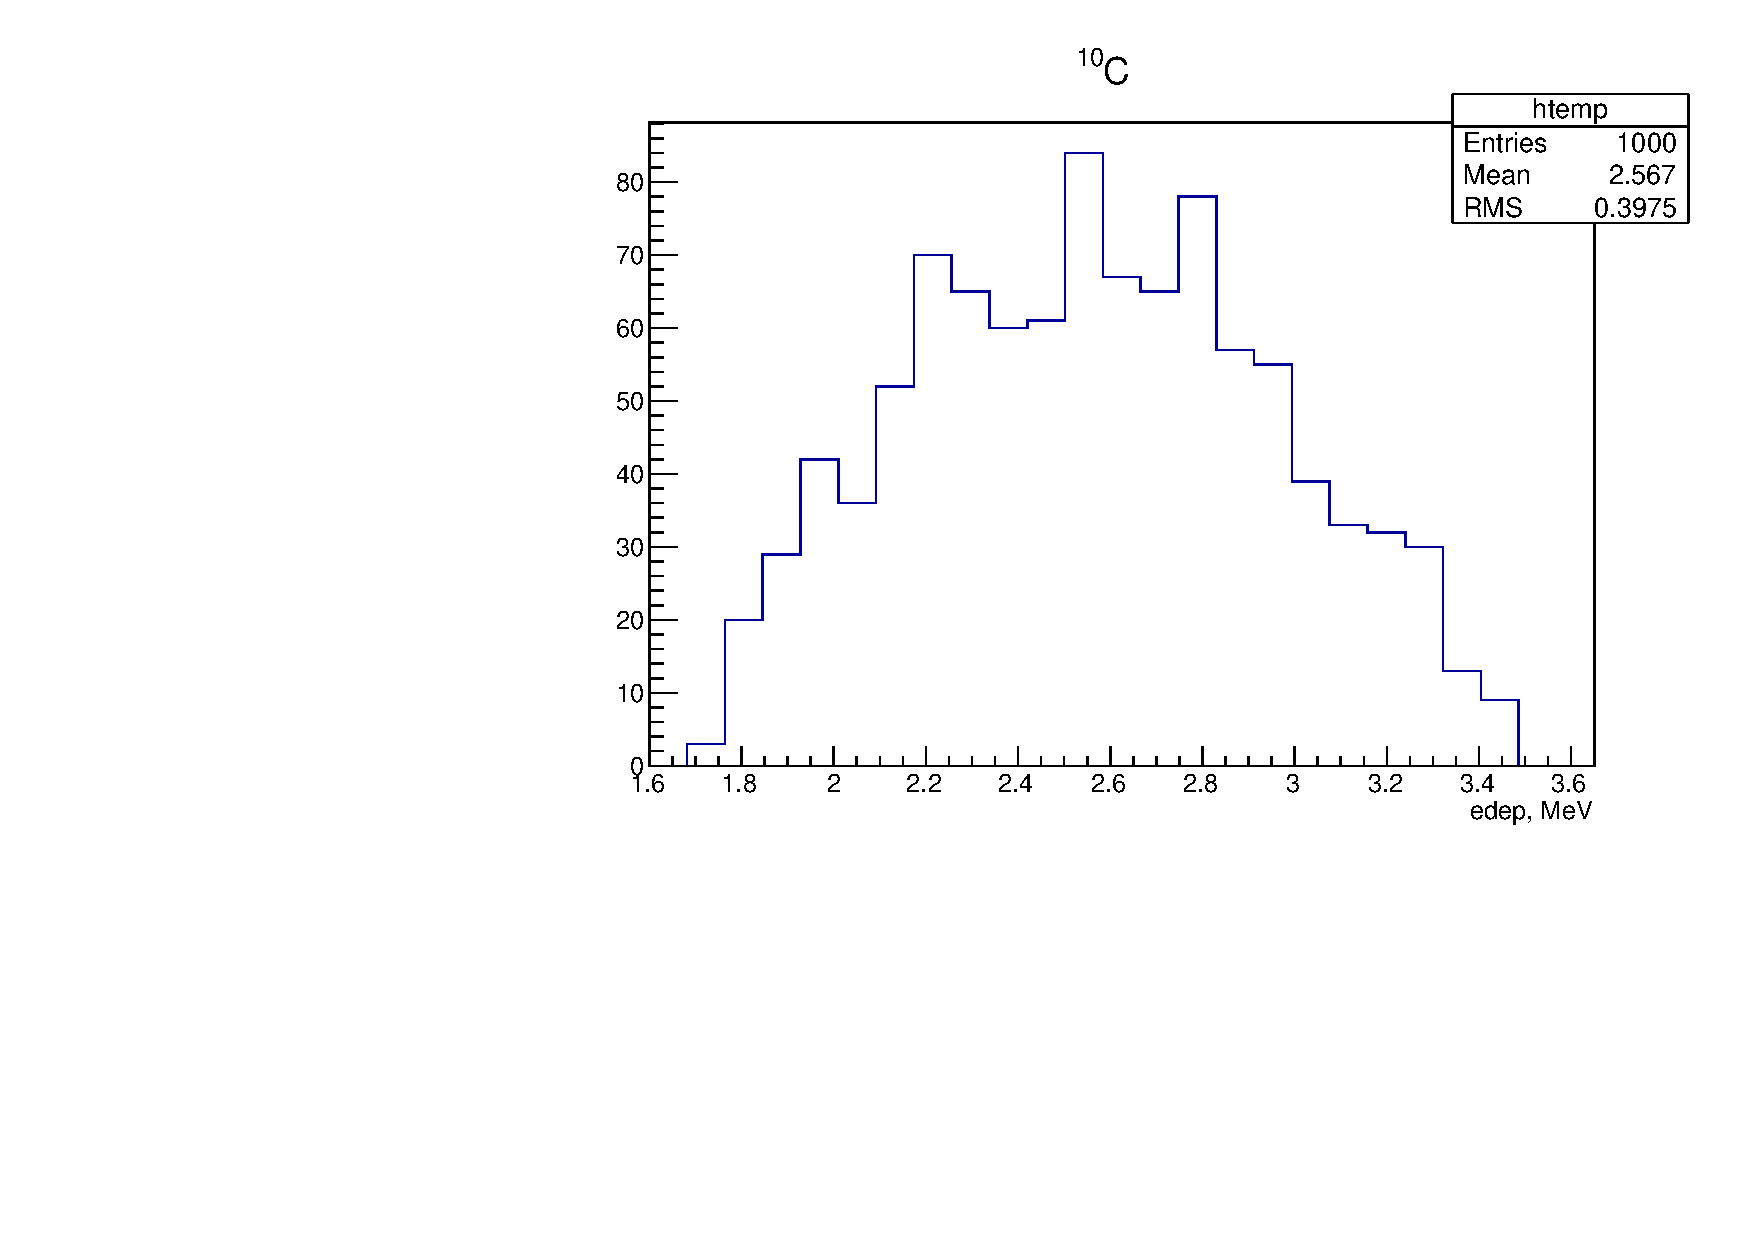
\includegraphics[width=0.95\textwidth]{hEdep_C10.pdf}
  \caption{Energy deposition in $^{10}$C events.}
  \label{fig:Edep_C10}
\end{figure}

\begin{figure}[h]
  \centering
  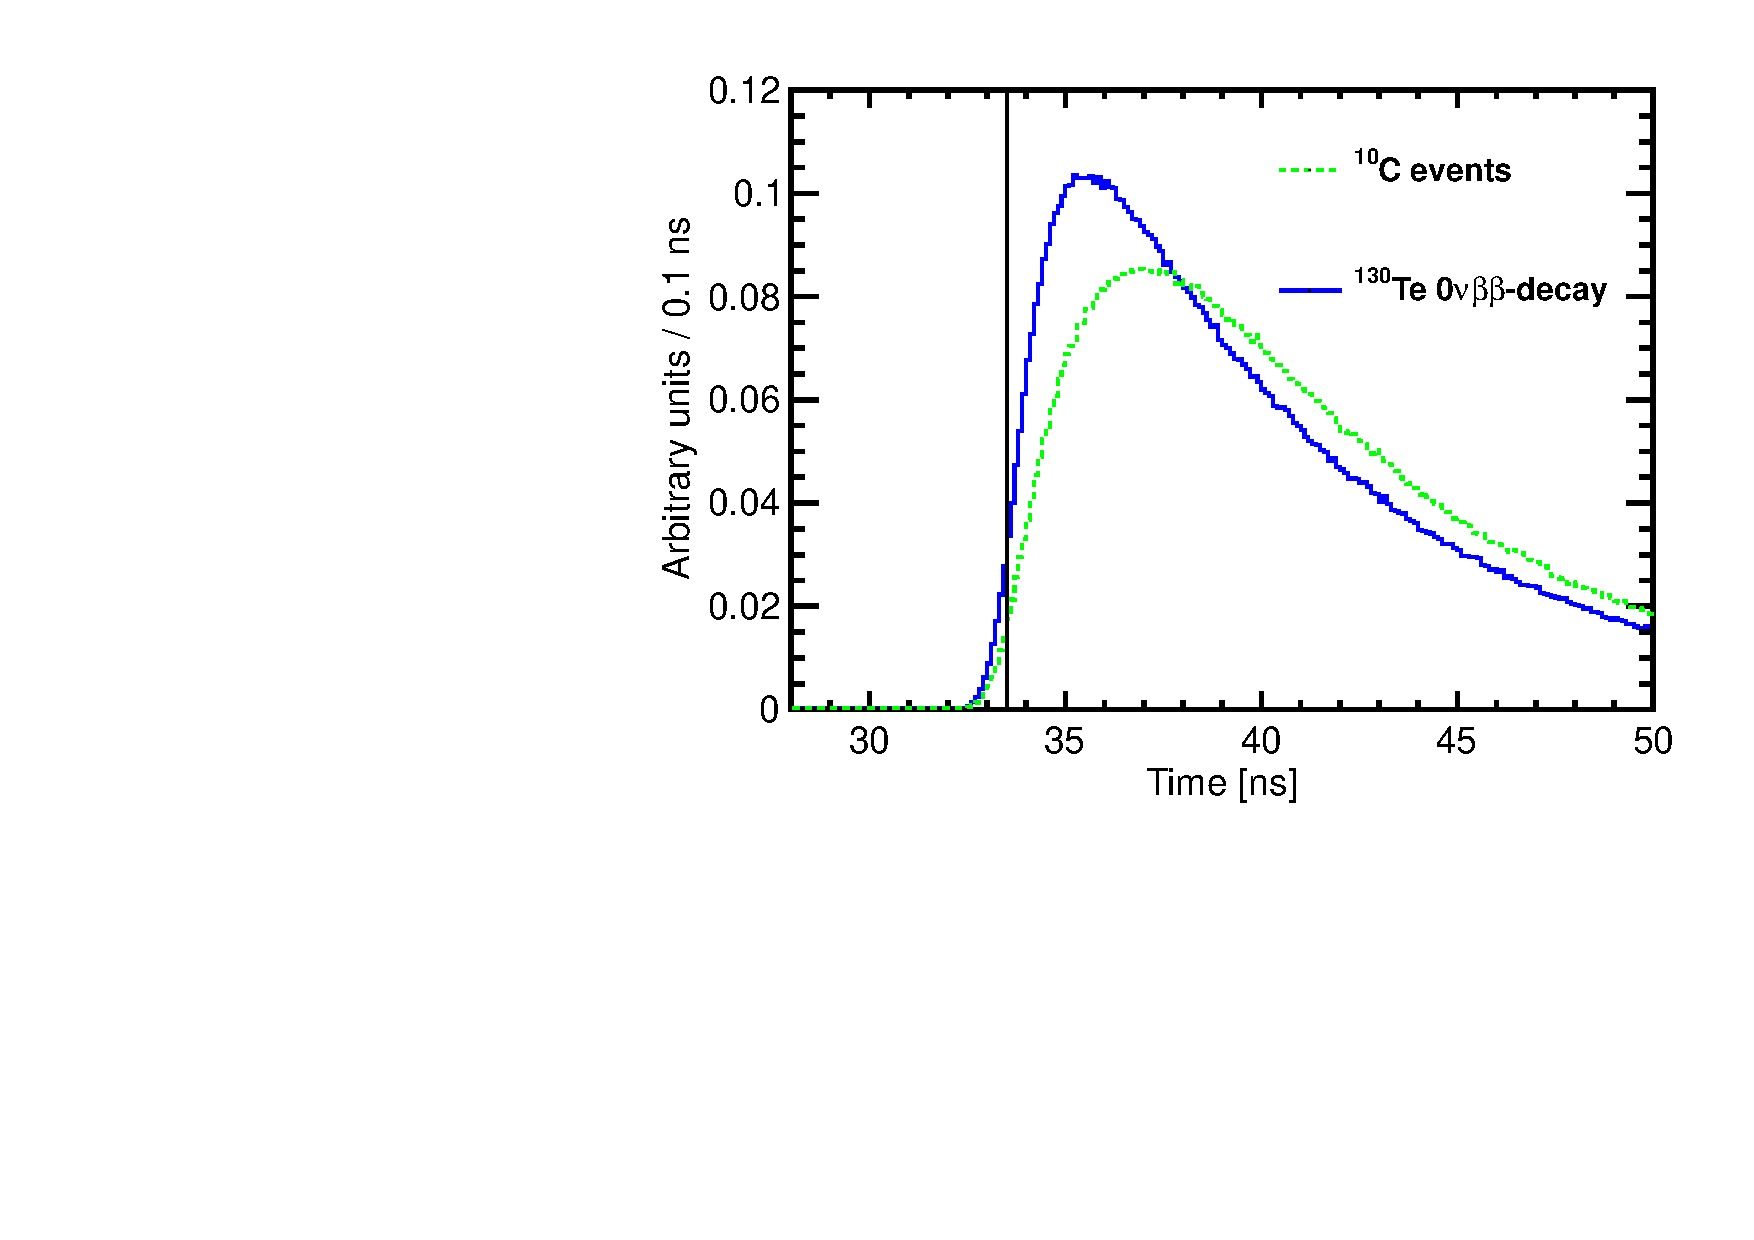
\includegraphics[width=0.45\textwidth]{hT_C10.pdf}
  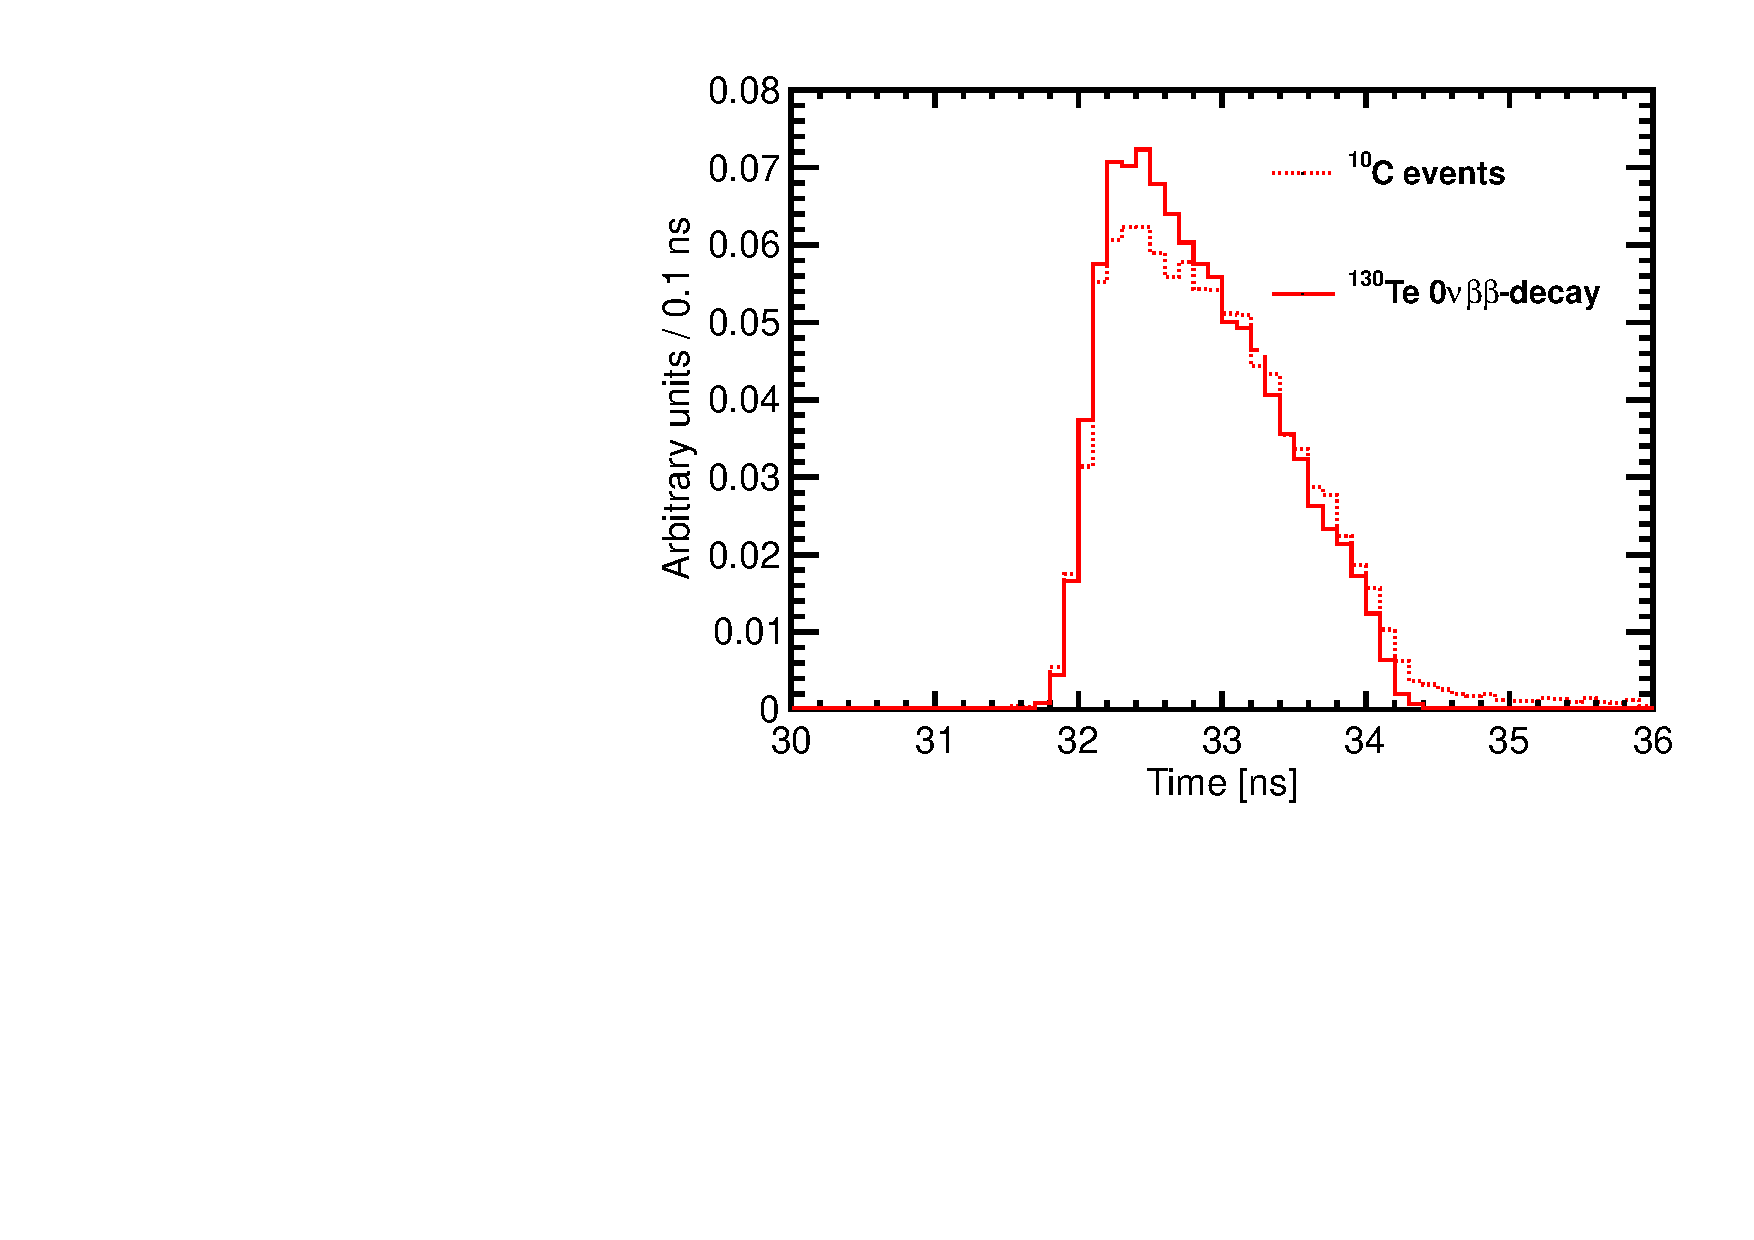
\includegraphics[width=0.45\textwidth]{hTche_C10.pdf}
  \caption{Photo-electron (PE) arrival times after application of the
    photo-detector transit time spread (TTS) of 100~ps for the
    simulation of 1000 0{\nbb} decay events of $^{130}$Te (\emph{solid
      lines}) and $^{10}$C (\emph{dotted lines}) events at the center
    of the detector. All distributions are normalized for shape
    comparison. {\bf Absolute number of PEs per event depends on the
      total energy deposited in the
      detector. Figure~\ref{fig:Edep_C10} shows energy deposited in
      the detector in $^{10}$C events.} \emph{Left:} Scintillation PEs
    arrival time. The black vertical line illustrates a time cut at
    33.5 ns. \emph{Right:} Cherenkov PEs arrival time.}
\label{fig:Arrival_time_C10}
\end{figure}

We note that 98\% of $^{10}$C decays through the excited state of
$^{10}$B(718), which has a half-life time of $\sim$1~ns. Therefore, the
majority of $^{10}$C events have a prompt positron accompanied by a
delayed 0.718~MeV gamma. This delayed gamma affects the PE arrival time
distribution. Figure~\ref{fig:Arrival_time_C10} compares the shape of the
PE arrival time distribution between $^{130}$Te 0{\nbb} decays and
$^{10}$C events. The time profile of the scintillation photons can be used
to separate signal from $^{10}$C events.

Samples of early photons are compared on Fig.~\ref{fig:NPhotDist_C10}

\begin{figure*}[ht]
  \centering
  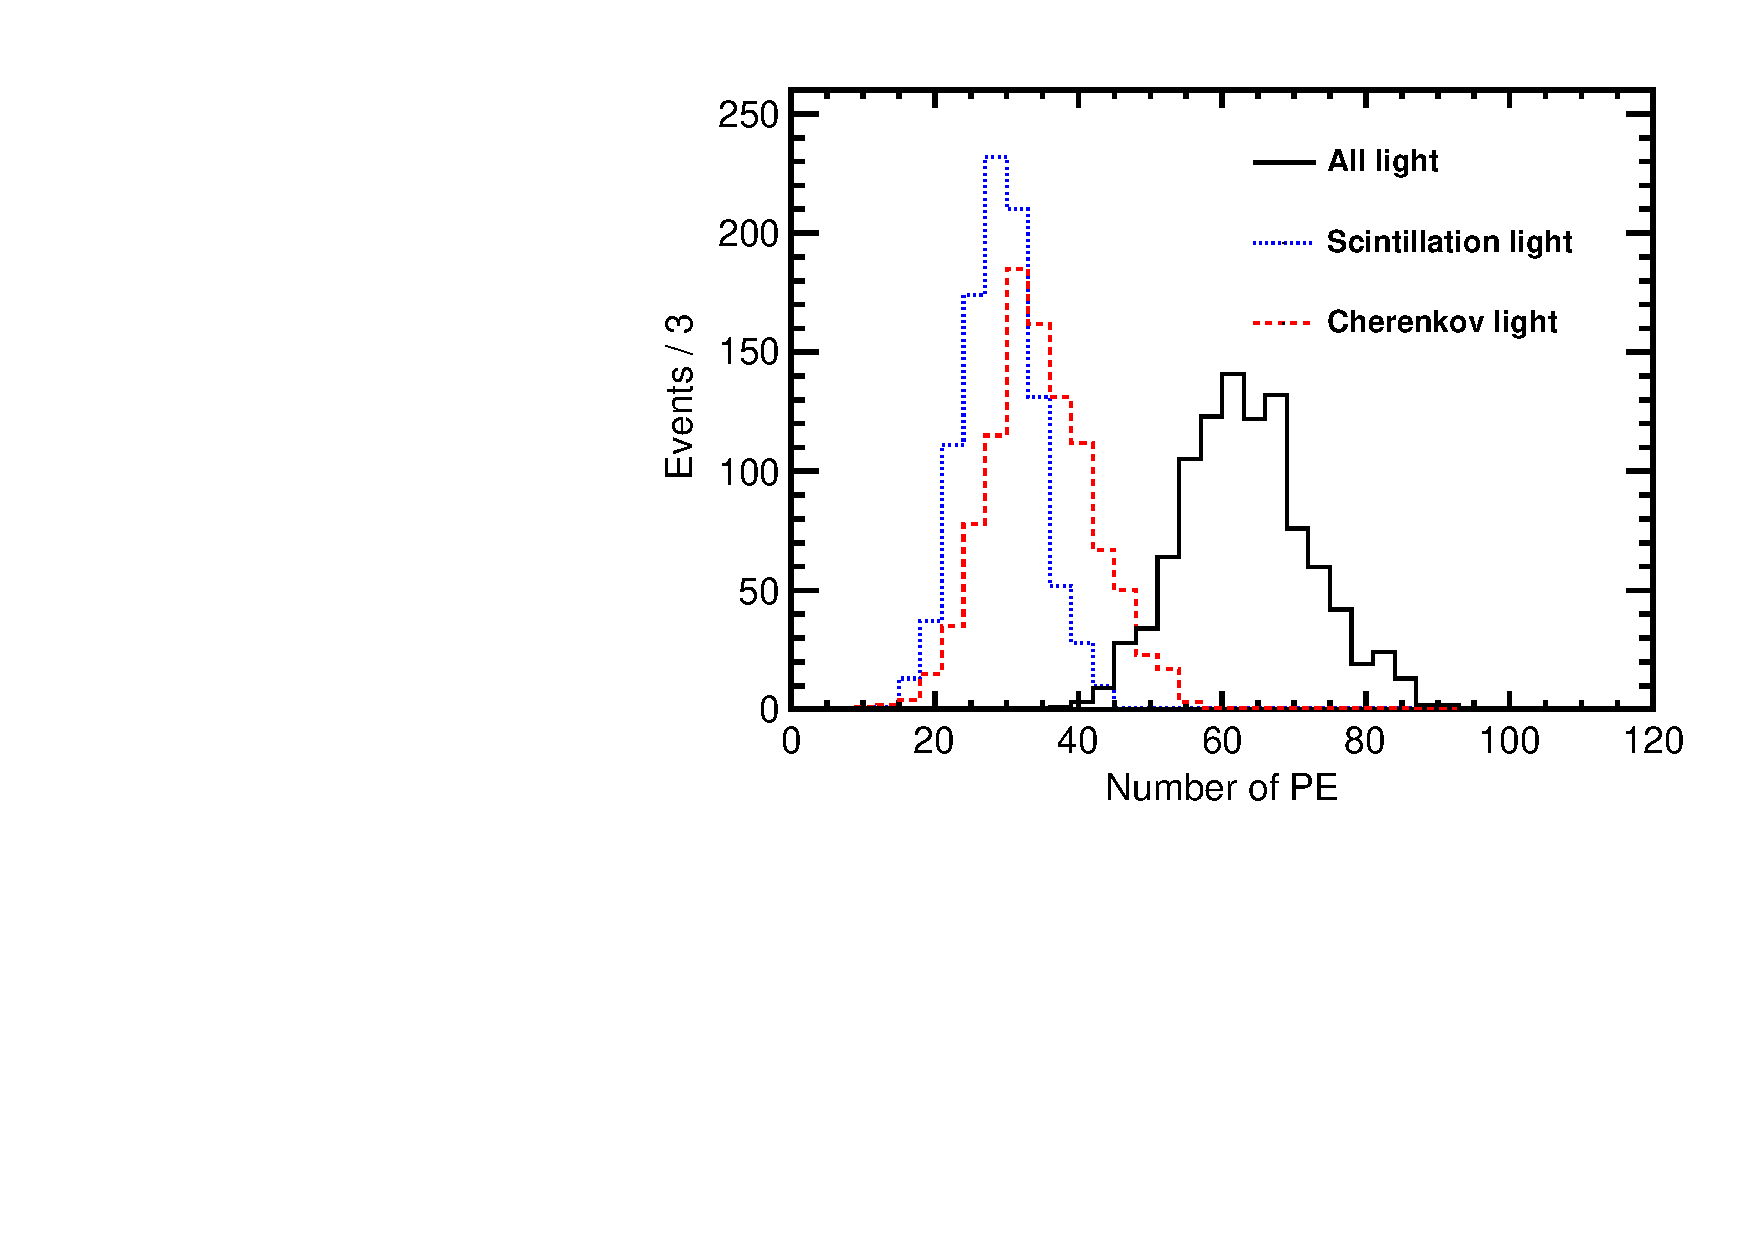
\includegraphics[width=0.45\textwidth]{hMomNPhot_Te130.pdf}
  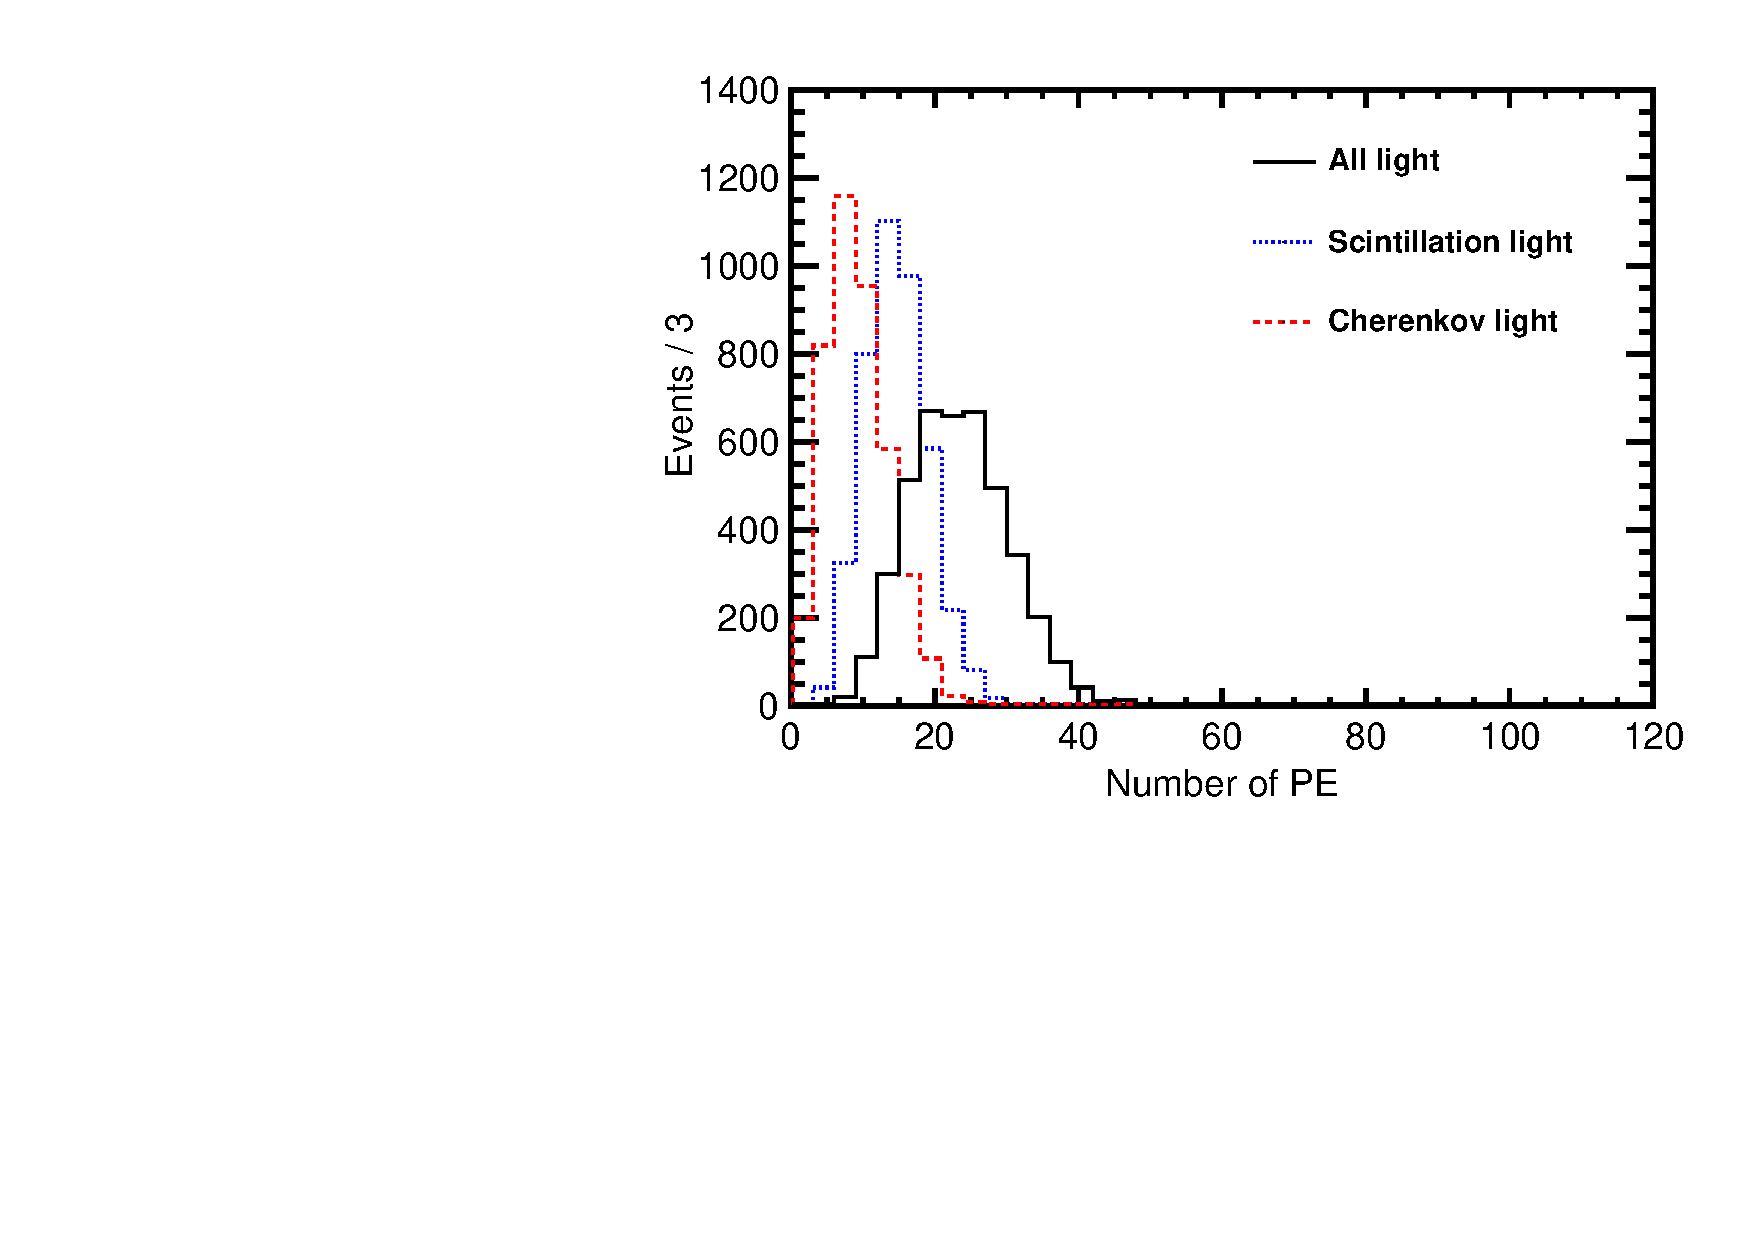
\includegraphics[width=0.45\textwidth]{hMomNPhot_C10.pdf}
  \caption{Early photons. Number of Cherenkov (\emph{dashed red line}), 
    scintillation
    (\emph{dotted blue line}), and total (\emph{solid black line}) PEs
    for the simulation of 1000 $^{130}$Te 0{\nbb} decay (left panel)
    and of 648 $^{10}$C (\emph{right panel}) events (1000 $^{10}$C events was 
    generated, but selected only those that has total energy deposition in the 
    detector in the range between 2.1 and 2.9~MeV).}
\label{fig:NPhotDist_C10}
\end{figure*}

Comparison of $S_0$ and $S_1$ distributions between 0{\nbb} decay and
$^{10}$C events is shown in Fig.~\ref{fig:S_vs_energy_C10}.

\begin{figure*}[h]
\centering
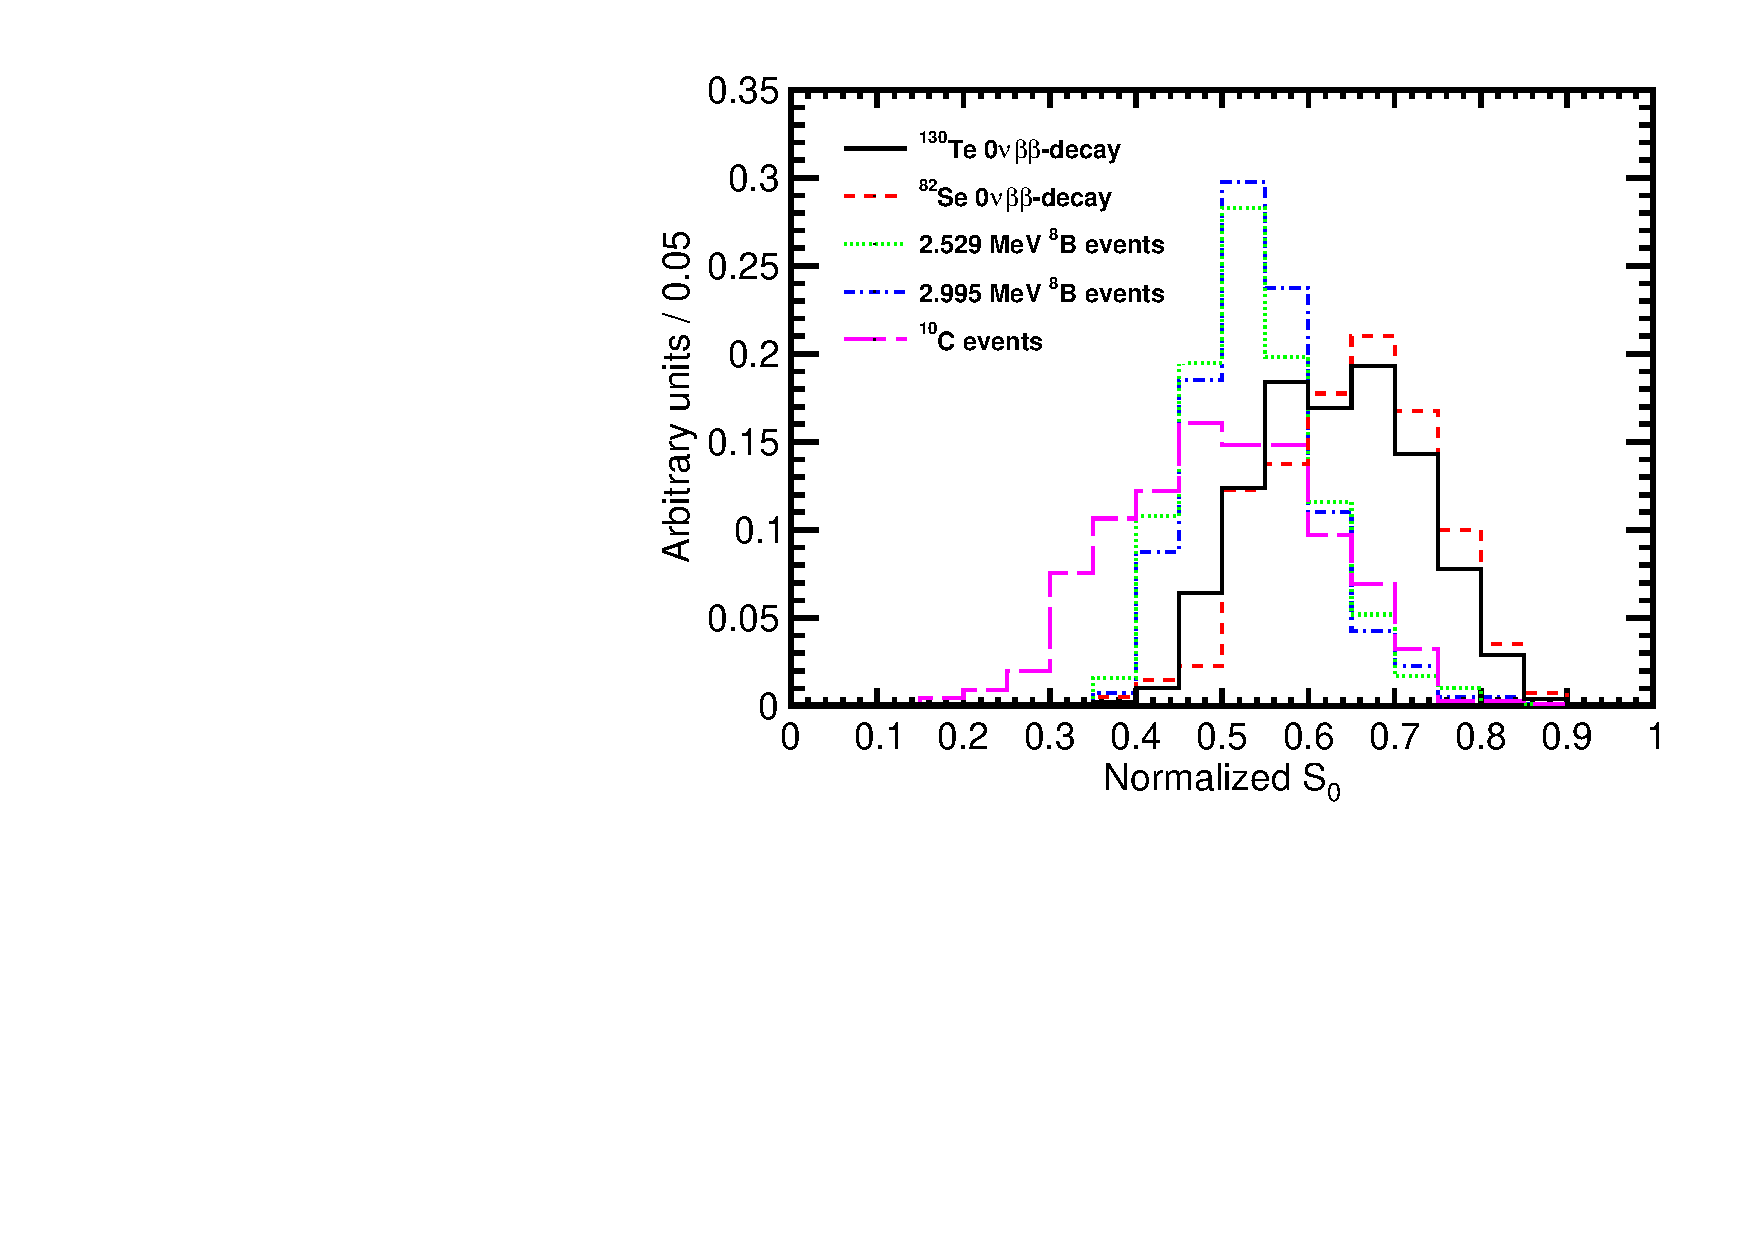
\includegraphics[width=0.49\textwidth]{hS0_C10.pdf}
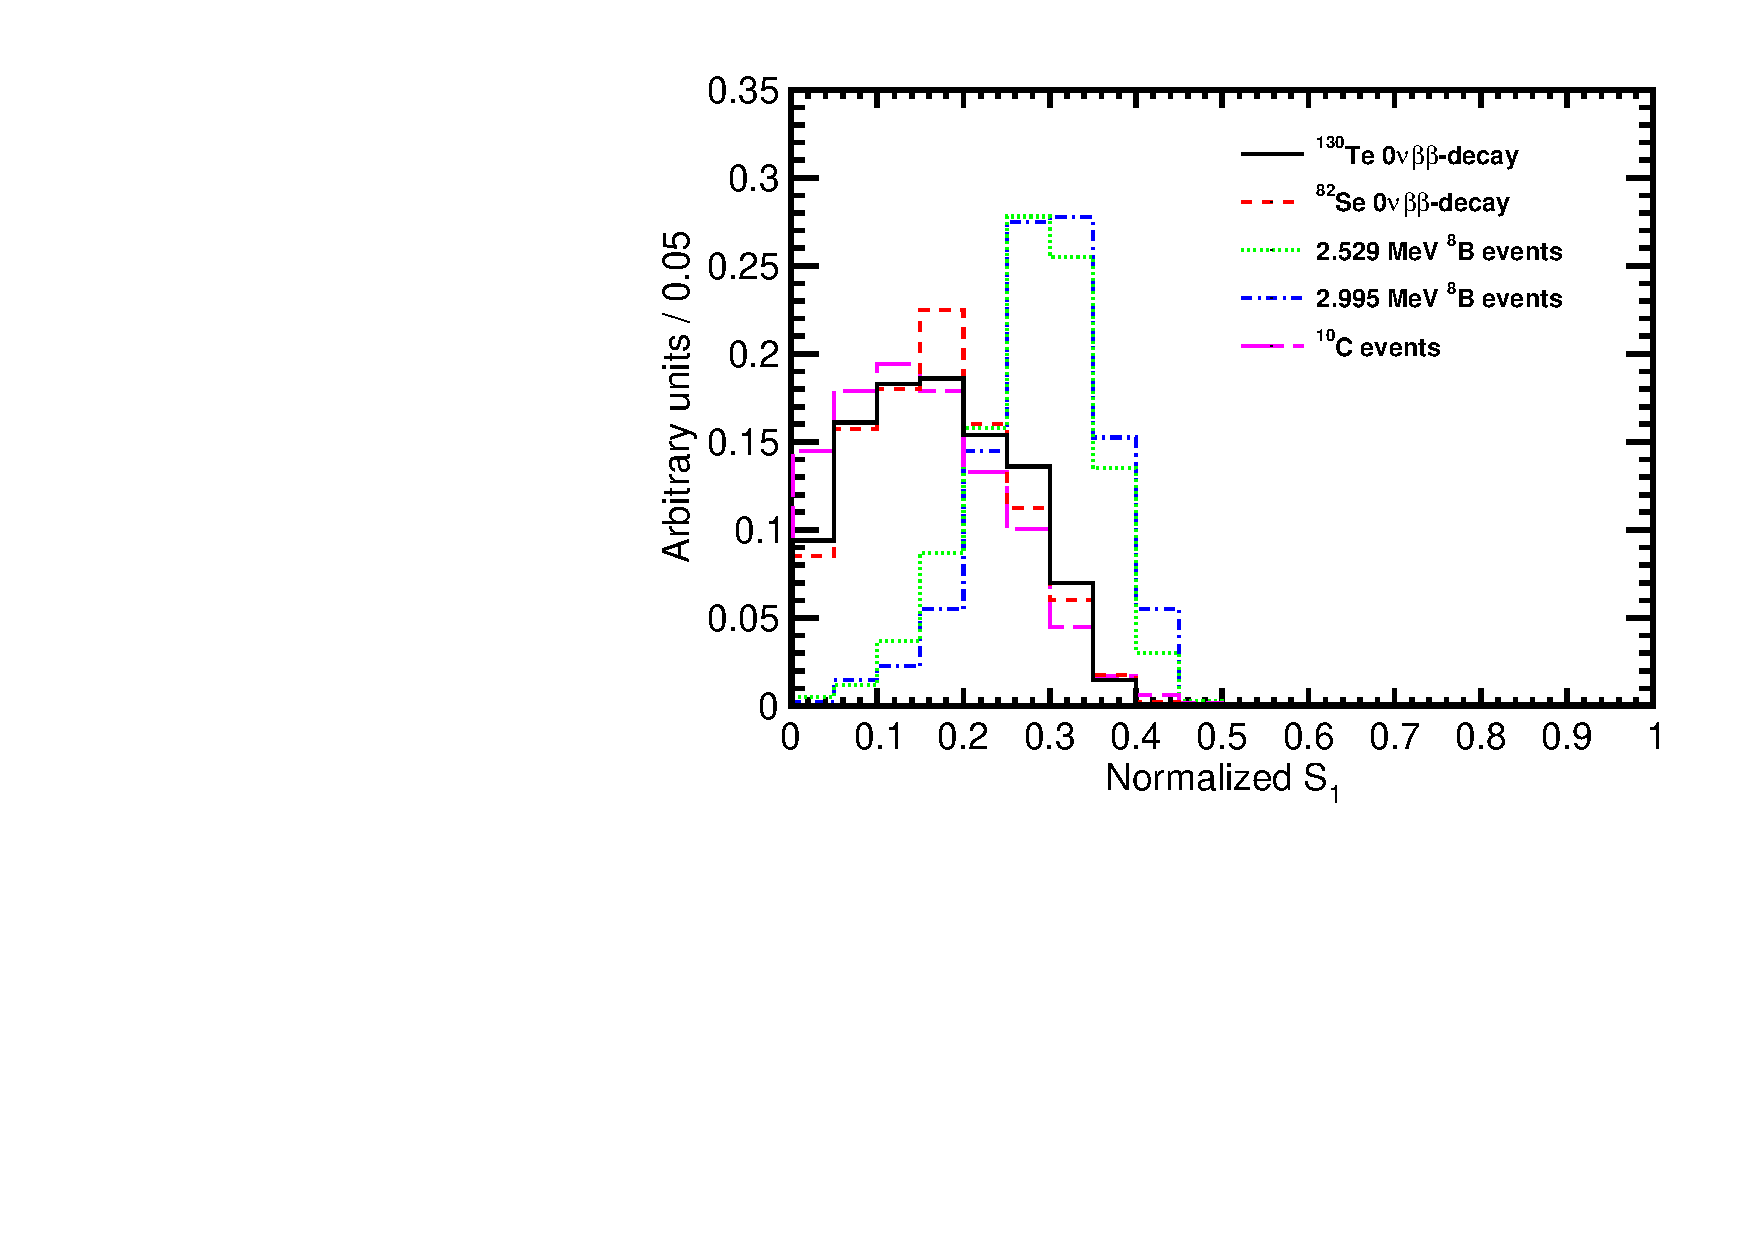
\includegraphics[width=0.49\textwidth]{hS1_C10.pdf}
\caption{$S_0$ (\emph{left}) and $S_1$ (\emph{right}) distributions
  for events with different event topologies. $^{130}$Te, $^{82}$Se 0{\nbb} 
  decays compared with $^{8}$B and $^{10}$C events. The simulation is done 
  for events with the vertex in the center of the detector. $^{8}$B events 
  are implemented as 2.529~MeV or 2.995~MeV electrons with initial direction 
  along $x$-axis. $^{10}$C events are selected in the energy range between 2.1 
  and 2.9~MeV. Perfect vertex reconstruction - true vertex position is used. 
  Time cut of 33.5~ns on the photon arrival time is applied.}
\label{fig:S_vs_energy}
\end{figure*}


\begin{figure}[h]
  \centering
  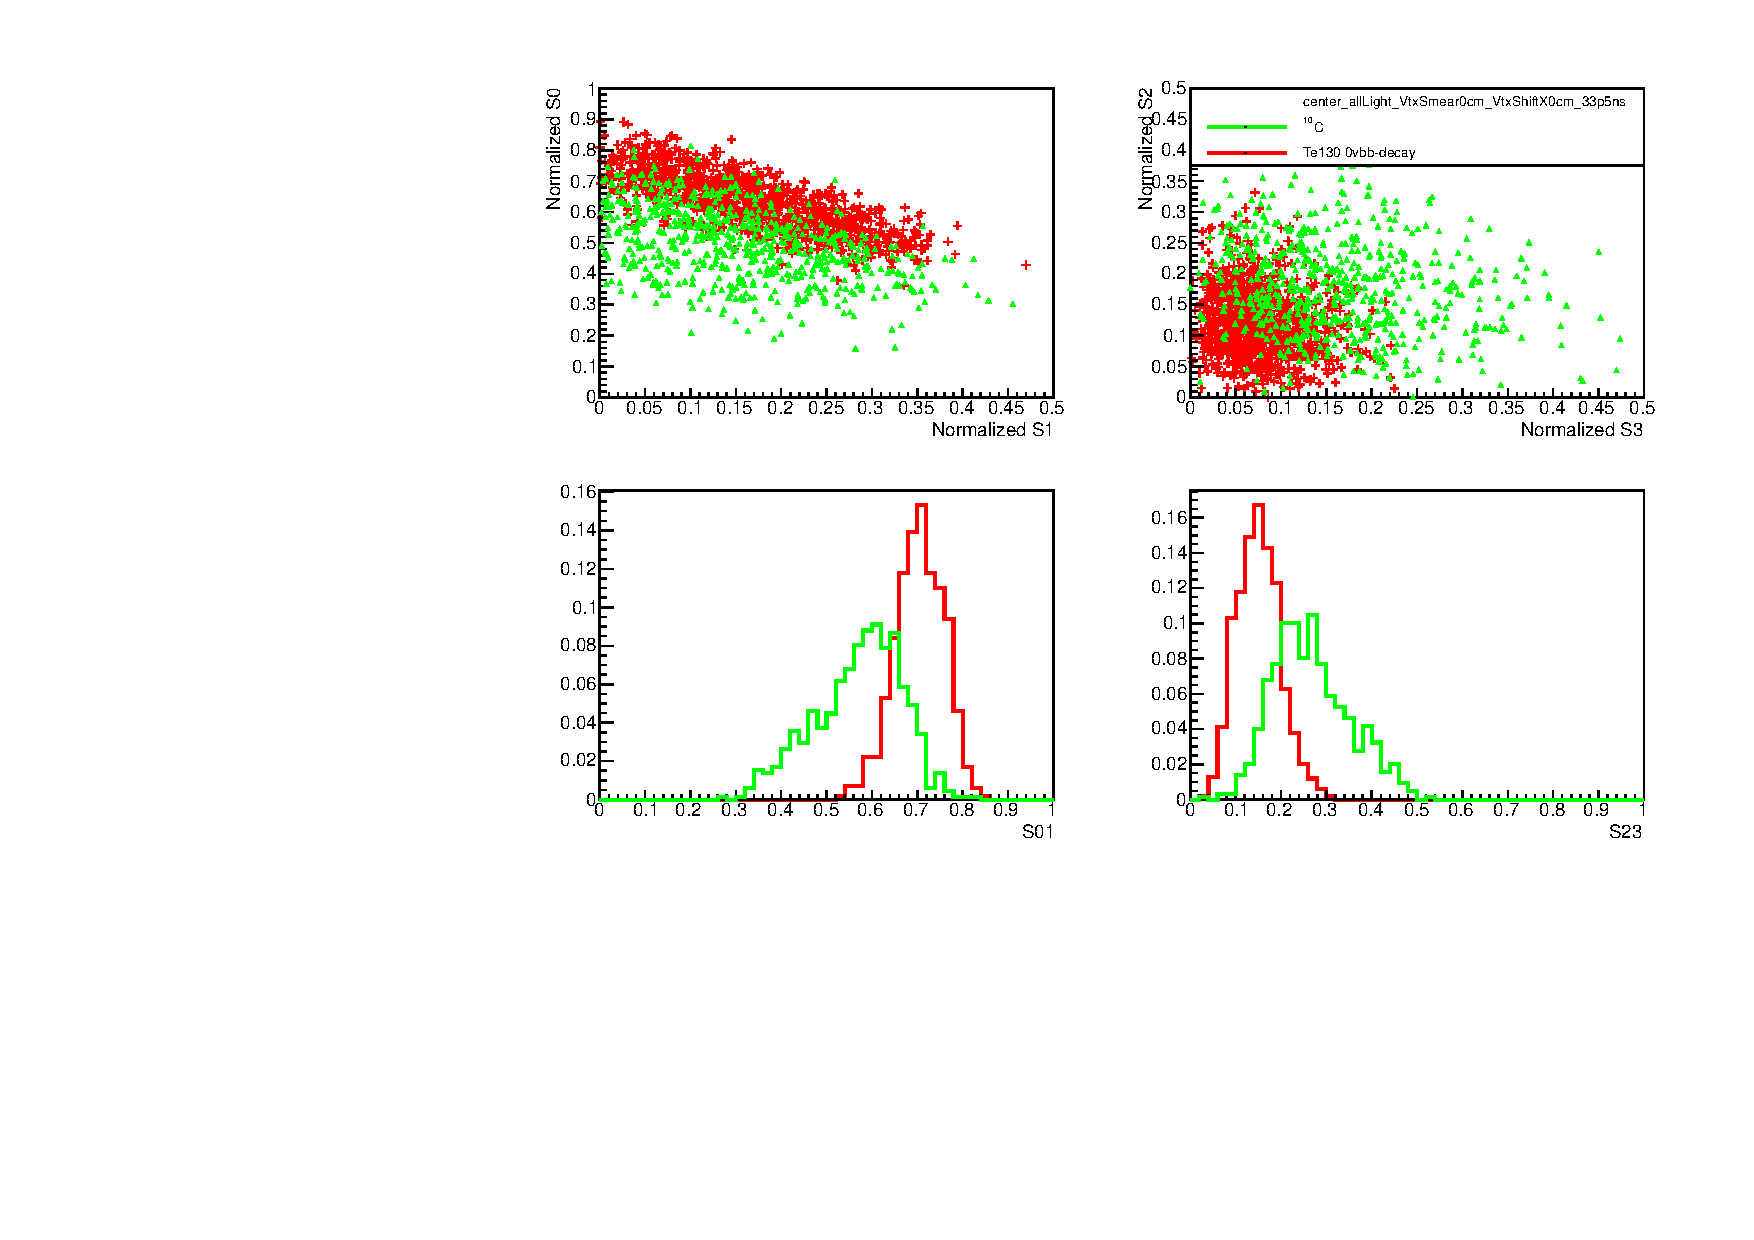
\includegraphics[width=0.95\textwidth]{hSLPlots_C10_allLight_VtxSmear0cm_VtxShiftX0cm_33p5ns_center.pdf}
  \caption{Spherical harmonics comparison between $^{130}$Te 0{\nbb}
    decay signal ($Q=2.529$~MeV) (\emph{red}) and $^{10}$C solar
    neutrinos background (blue) for 1000 simulated events originated
    at the center of the sphere. $^{10}$C with energy deposition
    between 2.1~MeV and 2.9~MeV are considered. Perfect vertex
    reconstruction - true vertex position is used. Time cut of 33.5~ns
    on the photon arrival time is applied. \emph{Top left:} S$_0$
    versus S$_1$ scatter plot. \emph{Top right:} S$_2$ versus S$_3$
    scatter plot. \emph{Bottom left:} Distribution of the
    S$^{C10}_{01}$ variable calculated for signal (\emph{red}) and
    background (\emph{green}). \emph{Bottom right:} Distribution of
    the S$^{C10}_{23}$ variable calculated for signal (\emph{red}) and
    background (\emph{green}).}
  \label{fig:SL_C10_33p5ns_center}
\end{figure}


Comparison of spherical harmonics is shown in
Fig.~\ref{fig:SL_C10_33p5ns_center}. $^{10}$C events are generated at
the center of the detector. True vertex position is used to apply a
33.5~ns time cut to select photons for the spherical harmonics
analysis. The separation is seen in S0 vs S1 and S2 vs S3 scatter
plots. We project both scatter plots to a line that gives maximum
separation (two bottom panels in Fig.~\ref{fig:SL_C10_33p5ns_center}).  
There is enough separation between the distributions to suggest that this analysis can be used to distinguish between 0{\nbb} and $^{10}$C events.

%\section{0{\nbb} decay vs backgrounds from Th and U series}
